%% fig_hankel.tex   (generated by make_round11.py; do not edit by hand)
%% The number that the corrected criterion asks of one complex.
\documentclass[tikz,border=8pt]{standalone}
\usepackage{amsmath,amssymb}
\usetikzlibrary{arrows.meta,calc,decorations.pathreplacing}
%% palette.tex -- shared colour definitions for the figures
\definecolor{PInk}{RGB}{26,32,44}
\definecolor{PBlue}{RGB}{37,82,139}
\definecolor{PTeal}{RGB}{23,127,125}
\definecolor{POchre}{RGB}{193,138,44}
\definecolor{PClay}{RGB}{178,74,58}
\definecolor{PSlate}{RGB}{108,122,137}
\definecolor{PViolet}{RGB}{110,86,150}
\definecolor{WBlue}{RGB}{223,234,246}
\definecolor{WTeal}{RGB}{220,238,236}
\definecolor{WOchre}{RGB}{250,240,218}
\definecolor{WClay}{RGB}{247,229,224}
\definecolor{WSlate}{RGB}{238,241,244}
\definecolor{PMag}{RGB}{158,58,110}
\definecolor{PGrass}{RGB}{62,124,66}
\definecolor{PAmber}{RGB}{214,112,38}
\definecolor{PIndigo}{RGB}{58,64,140}
\definecolor{PRule}{RGB}{176,186,197}

%% shared macros so the standalone figures match the paper
\providecommand{\QQ}{\mathbb{Q}}
\providecommand{\ZZ}{\mathbb{Z}}
\providecommand{\RR}{\mathbb{R}}
\providecommand{\CC}{\mathbb{C}}
\providecommand{\PP}{\mathbb{P}}
\providecommand{\Kx}{K^{\times}}
\providecommand{\HW}{W}
\providecommand{\Nm}{\mathrm{N}}
\providecommand{\Hdg}{\mathrm{Hdg}}
\providecommand{\NS}{\mathrm{NS}}
\providecommand{\cA}{\mathcal{A}}
\providecommand{\cD}{\mathcal{D}}
\providecommand{\cF}{\mathcal{F}}
\providecommand{\cP}{\mathcal{P}}
\providecommand{\cO}{\mathcal{O}}
\providecommand{\cQ}{\mathcal{Q}}
\providecommand{\bbar}[1]{\overline{#1}}
\providecommand{\ch}{\operatorname{ch}}
\providecommand{\End}{\mathrm{End}}

\begin{document}
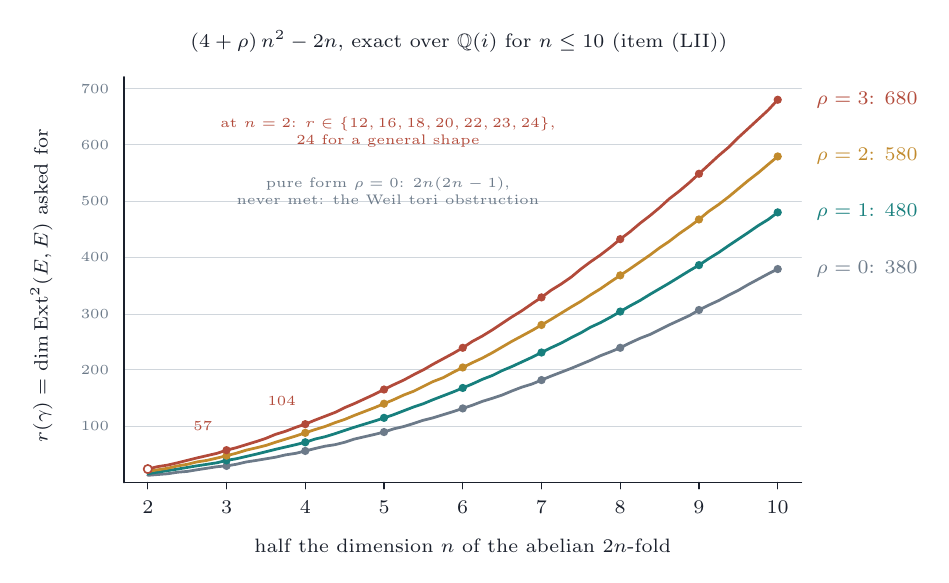
\begin{tikzpicture}[x=1cm,y=1cm,line join=round,line cap=round,
  font=\small,text=PInk]
  \draw[PRule!60,line width=0.30pt] (-0.30,0.71) -- (8.30,0.71);
  \node[text=PSlate,inner sep=1pt,align=center,font=\tiny,anchor=east] at (-0.45,0.71) {$100$};
  \draw[PRule!60,line width=0.30pt] (-0.30,1.43) -- (8.30,1.43);
  \node[text=PSlate,inner sep=1pt,align=center,font=\tiny,anchor=east] at (-0.45,1.43) {$200$};
  \draw[PRule!60,line width=0.30pt] (-0.30,2.14) -- (8.30,2.14);
  \node[text=PSlate,inner sep=1pt,align=center,font=\tiny,anchor=east] at (-0.45,2.14) {$300$};
  \draw[PRule!60,line width=0.30pt] (-0.30,2.86) -- (8.30,2.86);
  \node[text=PSlate,inner sep=1pt,align=center,font=\tiny,anchor=east] at (-0.45,2.86) {$400$};
  \draw[PRule!60,line width=0.30pt] (-0.30,3.57) -- (8.30,3.57);
  \node[text=PSlate,inner sep=1pt,align=center,font=\tiny,anchor=east] at (-0.45,3.57) {$500$};
  \draw[PRule!60,line width=0.30pt] (-0.30,4.29) -- (8.30,4.29);
  \node[text=PSlate,inner sep=1pt,align=center,font=\tiny,anchor=east] at (-0.45,4.29) {$600$};
  \draw[PRule!60,line width=0.30pt] (-0.30,5.00) -- (8.30,5.00);
  \node[text=PSlate,inner sep=1pt,align=center,font=\tiny,anchor=east] at (-0.45,5.00) {$700$};
  \draw[PInk,line width=0.60pt] (-0.30,0.00) -- (8.30,0.00);
  \draw[PInk,line width=0.60pt] (-0.30,0.00) -- (-0.30,5.15);
  \draw[PInk,line width=0.50pt] (0.00,0.00) -- (0.00,-0.08);
  \node[text=PInk,inner sep=1pt,align=center,font=\scriptsize] at (0.00,-0.32) {$2$};
  \draw[PInk,line width=0.50pt] (1.00,0.00) -- (1.00,-0.08);
  \node[text=PInk,inner sep=1pt,align=center,font=\scriptsize] at (1.00,-0.32) {$3$};
  \draw[PInk,line width=0.50pt] (2.00,0.00) -- (2.00,-0.08);
  \node[text=PInk,inner sep=1pt,align=center,font=\scriptsize] at (2.00,-0.32) {$4$};
  \draw[PInk,line width=0.50pt] (3.00,0.00) -- (3.00,-0.08);
  \node[text=PInk,inner sep=1pt,align=center,font=\scriptsize] at (3.00,-0.32) {$5$};
  \draw[PInk,line width=0.50pt] (4.00,0.00) -- (4.00,-0.08);
  \node[text=PInk,inner sep=1pt,align=center,font=\scriptsize] at (4.00,-0.32) {$6$};
  \draw[PInk,line width=0.50pt] (5.00,0.00) -- (5.00,-0.08);
  \node[text=PInk,inner sep=1pt,align=center,font=\scriptsize] at (5.00,-0.32) {$7$};
  \draw[PInk,line width=0.50pt] (6.00,0.00) -- (6.00,-0.08);
  \node[text=PInk,inner sep=1pt,align=center,font=\scriptsize] at (6.00,-0.32) {$8$};
  \draw[PInk,line width=0.50pt] (7.00,0.00) -- (7.00,-0.08);
  \node[text=PInk,inner sep=1pt,align=center,font=\scriptsize] at (7.00,-0.32) {$9$};
  \draw[PInk,line width=0.50pt] (8.00,0.00) -- (8.00,-0.08);
  \node[text=PInk,inner sep=1pt,align=center,font=\scriptsize] at (8.00,-0.32) {$10$};
  \node[text=PInk,inner sep=1pt,align=center,font=\scriptsize] at (4.00,-0.80) {half the dimension $n$ of the abelian $2n$-fold};
  \node[text=PInk,inner sep=1pt,align=center,font=\scriptsize,rotate=90] at (-1.35,2.50) {$r(\gamma)=\dim\mathrm{Ext}^{2}(E,E)$ asked for};
  \draw[PSlate,line width=1.00pt] (0.00,0.09) -- (0.12,0.10) -- (0.25,0.11) -- (0.38,0.13) -- (0.50,0.14) -- (0.62,0.16) -- (0.75,0.18) -- (0.88,0.20) -- (1.00,0.21) -- (1.12,0.23) -- (1.25,0.26) -- (1.38,0.28) -- (1.50,0.30) -- (1.62,0.32) -- (1.75,0.35) -- (1.88,0.37) -- (2.00,0.40) -- (2.12,0.43) -- (2.25,0.46) -- (2.38,0.48) -- (2.50,0.51) -- (2.62,0.55) -- (2.75,0.58) -- (2.88,0.61) -- (3.00,0.64) -- (3.12,0.68) -- (3.25,0.71) -- (3.38,0.75) -- (3.50,0.79) -- (3.62,0.82) -- (3.75,0.86) -- (3.88,0.90) -- (4.00,0.94) -- (4.12,0.98) -- (4.25,1.03) -- (4.38,1.07) -- (4.50,1.11) -- (4.62,1.16) -- (4.75,1.21) -- (4.88,1.25) -- (5.00,1.30) -- (5.12,1.35) -- (5.25,1.40) -- (5.38,1.45) -- (5.50,1.50) -- (5.62,1.55) -- (5.75,1.61) -- (5.88,1.66) -- (6.00,1.71) -- (6.12,1.77) -- (6.25,1.83) -- (6.38,1.88) -- (6.50,1.94) -- (6.62,2.00) -- (6.75,2.06) -- (6.88,2.12) -- (7.00,2.19) -- (7.12,2.25) -- (7.25,2.31) -- (7.38,2.38) -- (7.50,2.44) -- (7.62,2.51) -- (7.75,2.58) -- (7.88,2.65) -- (8.00,2.71);
  \fill[PSlate] (1.00,0.21) circle (1.5pt);
  \fill[PSlate] (2.00,0.40) circle (1.5pt);
  \fill[PSlate] (3.00,0.64) circle (1.5pt);
  \fill[PSlate] (4.00,0.94) circle (1.5pt);
  \fill[PSlate] (5.00,1.30) circle (1.5pt);
  \fill[PSlate] (6.00,1.71) circle (1.5pt);
  \fill[PSlate] (7.00,2.19) circle (1.5pt);
  \fill[PSlate] (8.00,2.71) circle (1.5pt);
  \node[text=PSlate,inner sep=1pt,align=center,font=\scriptsize,anchor=west] at (8.45,2.71) {$\rho=0$: $380$};
  \draw[PTeal,line width=1.00pt] (0.00,0.11) -- (0.12,0.13) -- (0.25,0.15) -- (0.38,0.17) -- (0.50,0.19) -- (0.62,0.21) -- (0.75,0.23) -- (0.88,0.25) -- (1.00,0.28) -- (1.12,0.30) -- (1.25,0.33) -- (1.38,0.36) -- (1.50,0.39) -- (1.62,0.42) -- (1.75,0.45) -- (1.88,0.48) -- (2.00,0.51) -- (2.12,0.55) -- (2.25,0.58) -- (2.38,0.62) -- (2.50,0.66) -- (2.62,0.70) -- (2.75,0.74) -- (2.88,0.78) -- (3.00,0.82) -- (3.12,0.86) -- (3.25,0.91) -- (3.38,0.96) -- (3.50,1.00) -- (3.62,1.05) -- (3.75,1.10) -- (3.88,1.15) -- (4.00,1.20) -- (4.12,1.25) -- (4.25,1.31) -- (4.38,1.36) -- (4.50,1.42) -- (4.62,1.47) -- (4.75,1.53) -- (4.88,1.59) -- (5.00,1.65) -- (5.12,1.71) -- (5.25,1.77) -- (5.38,1.84) -- (5.50,1.90) -- (5.62,1.97) -- (5.75,2.03) -- (5.88,2.10) -- (6.00,2.17) -- (6.12,2.24) -- (6.25,2.31) -- (6.38,2.39) -- (6.50,2.46) -- (6.62,2.53) -- (6.75,2.61) -- (6.88,2.69) -- (7.00,2.76) -- (7.12,2.84) -- (7.25,2.92) -- (7.38,3.01) -- (7.50,3.09) -- (7.62,3.17) -- (7.75,3.26) -- (7.88,3.34) -- (8.00,3.43);
  \fill[PTeal] (1.00,0.28) circle (1.5pt);
  \fill[PTeal] (2.00,0.51) circle (1.5pt);
  \fill[PTeal] (3.00,0.82) circle (1.5pt);
  \fill[PTeal] (4.00,1.20) circle (1.5pt);
  \fill[PTeal] (5.00,1.65) circle (1.5pt);
  \fill[PTeal] (6.00,2.17) circle (1.5pt);
  \fill[PTeal] (7.00,2.76) circle (1.5pt);
  \fill[PTeal] (8.00,3.43) circle (1.5pt);
  \node[text=PTeal,inner sep=1pt,align=center,font=\scriptsize,anchor=west] at (8.45,3.43) {$\rho=1$: $480$};
  \draw[POchre,line width=1.00pt] (0.00,0.14) -- (0.12,0.16) -- (0.25,0.18) -- (0.38,0.21) -- (0.50,0.23) -- (0.62,0.26) -- (0.75,0.28) -- (0.88,0.31) -- (1.00,0.34) -- (1.12,0.37) -- (1.25,0.41) -- (1.38,0.44) -- (1.50,0.47) -- (1.62,0.51) -- (1.75,0.55) -- (1.88,0.59) -- (2.00,0.63) -- (2.12,0.67) -- (2.25,0.71) -- (2.38,0.76) -- (2.50,0.80) -- (2.62,0.85) -- (2.75,0.90) -- (2.88,0.95) -- (3.00,1.00) -- (3.12,1.05) -- (3.25,1.11) -- (3.38,1.16) -- (3.50,1.22) -- (3.62,1.28) -- (3.75,1.33) -- (3.88,1.40) -- (4.00,1.46) -- (4.12,1.52) -- (4.25,1.58) -- (4.38,1.65) -- (4.50,1.72) -- (4.62,1.79) -- (4.75,1.86) -- (4.88,1.93) -- (5.00,2.00) -- (5.12,2.07) -- (5.25,2.15) -- (5.38,2.23) -- (5.50,2.30) -- (5.62,2.38) -- (5.75,2.46) -- (5.88,2.55) -- (6.00,2.63) -- (6.12,2.71) -- (6.25,2.80) -- (6.38,2.89) -- (6.50,2.98) -- (6.62,3.06) -- (6.75,3.16) -- (6.88,3.25) -- (7.00,3.34) -- (7.12,3.44) -- (7.25,3.53) -- (7.38,3.63) -- (7.50,3.73) -- (7.62,3.83) -- (7.75,3.93) -- (7.88,4.04) -- (8.00,4.14);
  \fill[POchre] (1.00,0.34) circle (1.5pt);
  \fill[POchre] (2.00,0.63) circle (1.5pt);
  \fill[POchre] (3.00,1.00) circle (1.5pt);
  \fill[POchre] (4.00,1.46) circle (1.5pt);
  \fill[POchre] (5.00,2.00) circle (1.5pt);
  \fill[POchre] (6.00,2.63) circle (1.5pt);
  \fill[POchre] (7.00,3.34) circle (1.5pt);
  \fill[POchre] (8.00,4.14) circle (1.5pt);
  \node[text=POchre,inner sep=1pt,align=center,font=\scriptsize,anchor=west] at (8.45,4.14) {$\rho=2$: $580$};
  \draw[PClay,line width=1.00pt] (0.00,0.17) -- (0.12,0.20) -- (0.25,0.22) -- (0.38,0.25) -- (0.50,0.28) -- (0.62,0.31) -- (0.75,0.34) -- (0.88,0.37) -- (1.00,0.41) -- (1.12,0.44) -- (1.25,0.48) -- (1.38,0.52) -- (1.50,0.56) -- (1.62,0.61) -- (1.75,0.65) -- (1.88,0.70) -- (2.00,0.74) -- (2.12,0.79) -- (2.25,0.84) -- (2.38,0.89) -- (2.50,0.95) -- (2.62,1.00) -- (2.75,1.06) -- (2.88,1.12) -- (3.00,1.18) -- (3.12,1.24) -- (3.25,1.30) -- (3.38,1.37) -- (3.50,1.43) -- (3.62,1.50) -- (3.75,1.57) -- (3.88,1.64) -- (4.00,1.71) -- (4.12,1.79) -- (4.25,1.86) -- (4.38,1.94) -- (4.50,2.02) -- (4.62,2.10) -- (4.75,2.18) -- (4.88,2.27) -- (5.00,2.35) -- (5.12,2.44) -- (5.25,2.52) -- (5.38,2.61) -- (5.50,2.71) -- (5.62,2.80) -- (5.75,2.89) -- (5.88,2.99) -- (6.00,3.09) -- (6.12,3.18) -- (6.25,3.29) -- (6.38,3.39) -- (6.50,3.49) -- (6.62,3.60) -- (6.75,3.70) -- (6.88,3.81) -- (7.00,3.92) -- (7.12,4.03) -- (7.25,4.15) -- (7.38,4.26) -- (7.50,4.38) -- (7.62,4.49) -- (7.75,4.61) -- (7.88,4.73) -- (8.00,4.86);
  \fill[PClay] (1.00,0.41) circle (1.5pt);
  \fill[PClay] (2.00,0.74) circle (1.5pt);
  \fill[PClay] (3.00,1.18) circle (1.5pt);
  \fill[PClay] (4.00,1.71) circle (1.5pt);
  \fill[PClay] (5.00,2.35) circle (1.5pt);
  \fill[PClay] (6.00,3.09) circle (1.5pt);
  \fill[PClay] (7.00,3.92) circle (1.5pt);
  \fill[PClay] (8.00,4.86) circle (1.5pt);
  \node[text=PClay,inner sep=1pt,align=center,font=\scriptsize,anchor=west] at (8.45,4.86) {$\rho=3$: $680$};
  \node[text=PClay,inner sep=1pt,align=center,font=\tiny] at (0.70,0.71) {$57$};
  \node[text=PClay,inner sep=1pt,align=center,font=\tiny] at (1.70,1.04) {$104$};
  \draw[PClay,fill=white,line width=0.6pt] (0.00,0.17) circle (1.5pt);
  \node[text=PInk,inner sep=1pt,align=center,font=\scriptsize] at (3.95,5.60) {$(4+\rho)\,n^{2}-2n$, exact over $\QQ(i)$ for $n\le10$ (item (LII))};
  \node[text=PClay,inner sep=1pt,align=center,font=\tiny] at (3.05,4.45) {at $n=2$: $r\in\{12,16,18,20,22,23,24\}$,\\$24$ for a general shape};
  \node[text=PSlate,inner sep=1pt,align=center,font=\tiny] at (3.05,3.70) {pure form $\rho=0$: $2n(2n-1)$,\\never met: the Weil tori obstruction};
\end{tikzpicture}
\end{document}
